\chapter{绪论}

\section{研究背景}

%%%%%%%%  引入
如今,虚拟现实(Virtual Reality,VR)和增强现实(Augmented Reality,AR)等沉浸式技术正在快速发展,一定程度上改变了个人、企业与数字世界的互动方式,并给人们带来体验全新世界的可能。增强现实在真实场景的基础上,叠加计算机模拟产生的虚拟物体、场景,呈现给用户更具沉浸感的新体验。一个完整的身临其境的体验需要将视觉、听觉、触觉、嗅觉、味觉等多种感官融合到一个场景中。目前,增强现实技术大部分集中在视觉方面,例如谷歌眼镜。但是相比于视觉,声音能够更好地带来身临其境的体验,因为人可以感知任意方向的声学信息,而无需转向信号源~\tcite{book_immersive}。
% 当其他感官信息改变时,声音可以提供一个固定的场景,例如电影中不断变换视角,通过声音使听者处于一个固定的位置。

% 自然的听音环境可以定义为我们日常生活中所涉及的声音空间,世界上所有声音的本质都是三维的。听觉上的沉浸感指的是声音从四面八方从听者周围传来,这通常是人类在自然听音环境中的必然结果。
世界上所有声音的本质都是三维~(3D)~的,包含空间信息,然而在过去的大部分时间里,人类对~3D~声音的研究和使用集中在建筑声学和音乐创作方面。自~19~世纪以来,更先进的技术允许出现更具沉浸式的声音,目标可能是重现一个完整的声学环境,尽可能接近真实世界,也可能是创造一种新体验,对真实世界进行增强~\tcite{wenZhang_review}。我们可以捕捉、处理、存储和传输来自自然环境的声音,并通过使用扬声器或耳机进行回放以代替或增强自然聆听环境,这将有助于听者的听觉体验。
空间音频技术,特别是~3D~音频,可以再现身临其境的声音体验,已经成为信号与信息处理和人工智能领域的研究热点。从某种意义上来说,这个领域的迅速发展试图重新建立声音和空间之间的联系,而这种联系在某种程度上被早期的录音和复制的技术限制所切断~\tcite{book_immersive}。


空间音频重建技术可以分为双耳音频重建技术和声场重建技术,其区别主要在于是否考虑人的影响。其中,声场重建技术从单通道到立体声,再到多通道环绕声,最后到全息声。其最终目标是通过扬声器阵列在某一空间区域内再现自然的全景虚拟声场,尽可能保留原有声音的空间特性。
双耳音频重建技术,即双耳渲染技术,利用和模仿人耳听觉系统对空间音频的感知,通过耳机或扬声器,针对听者的双耳模拟再现虚拟的听觉环境~\tcite{wenZhang_review}。% 这句话的原因是张雯老师这个review中摘要说到:双耳录制和渲染是为了模仿人的双耳听觉系统,专门为听者的双耳进行重现,引言中第二段出现:双耳录制和渲染是指在双耳处录制和重现声场[1,2]。它的设计类似于人的双耳听觉系统,通常是用耳机[3,4]或几个扬声器[5,6],即,立体声扬声器。
这就产生了一种“你在那里”的第一人称视角,与声场重建技术中“他们在这里”的扬声器系统形成对比,体现了双耳音频技术的优越性~\tcite{book_immersive}。


本课题聚焦于双耳渲染技术,考虑人耳听觉系统,通过给听者提供空间听觉信息,再现具有高度真实感的三维听觉场景。
几十年来,这项技术一直受到科学界众多学者的广泛关注,在虚拟声学、建筑声学、语音通信、信息系统、媒体社交、教育和游戏娱乐等领域有着广泛的应用。


%%%%%%%%%%%%%%%%%%%%  双耳的应用展望
\newpage

当双耳渲染技术足够成熟时,其应用包括:
\begin{itemize}[leftmargin=*]
\item 提高语言通信的可懂度。目前绝大部分的语言通信采用的是单通路的信号传输系统,不能实现目标语言声源与其他声源在空间上分离,因而语言可懂度会变差。如果引入双耳渲染技术,对原始场景进行重现保留声源的空间信息,就可以提高语言通信的质量;
\item 引导视觉定位。声音信息的空间化可以引导视觉定位,甚至可以在不借助视觉的情况下寻找目标,从而减少寻找目标以及采取应对措施的时间,提高安全性。主要用途是民用或军用救援搜索、旅游或博物馆向导、盲人的导向和信息系统;
\item 减轻视觉负担。当目标的位置超出视觉的范围(如后方的目标),或同时有多个视觉目标时,可以结合双耳渲染技术,将部分目标信息转换成声音的空间信息重放出来,减轻视觉的负担;
\item 改变我们聆听音乐、与音乐互动、共存的方式,可以重新定义我们娱乐、交流和合作的方式,改善生活质量。
\end{itemize}


%  在多媒体系统中主要有两方面的应用,其一是双耳渲染技术能其二是多媒体计算机是组合实现虚拟现实和信息通信与处理、声视频娱乐功能的一个理想环境,而各种移动和手持设备可能会成为今后的重要应用方向。移动产品可能会集成语言通信、交互虚拟听觉环境、视像会议、信息导向、娱乐等多种功能,多媒体技术的应用也对空间声信号的压缩和传输提出了新的要求,将双耳渲染与空间音频编码技术相结合,以减少信号的码率和简化信号处理。

%%%%%%%%%%

双耳渲染技术是给听众提供空间音频的一种有效的方式。此外,虚拟听觉环境的音质和能否带来有效的真实感,对听者来说也变得越来越重要。到目前为止,双耳渲染技术得到了快速发展,但仍有许多挑战和待解决的问题。% \textbf{本段再修一下}

\section{国内外研究现状}

%%%%%%%% 实现 : 扬声器  或  耳机 ,实在多的话可以放在发展现状前端

双耳渲染技术的实现有两种方式: 基于耳机的双耳渲染和基于扬声器的双耳渲染。其中,通过耳机将双耳信号直接传输至听者耳膜是最自然和有效的方法。基于耳机的双耳渲染有很多优点:

% 再现双耳信号的终极目标是在听者的耳膜上重新产生一种相当于听者在自然听力条件下所听到的声音信号。将信号直接传输到听者的耳朵是传递高质量空间音频信号最直接和有效的方式。耳机是实现这一目标最方便和首选的再现方法,基于耳机的双耳信号重现有很多优点,其中最大的优点是提供了一个可控的聆听环境。
\begin{itemize}[leftmargin=*]
\item 具有完美的通道分离特性。耳机将左声道信号直接发送到左耳,右声道信号直接发送到右耳,因此到达每只耳朵的信号是独立呈现的,可以防止任何串音信号到达非预期的耳朵;
\item 较小的噪声干扰。除非严格控制,否则任何听力环境都含有背景噪声,这些噪声会叠加在重建的双耳信号上,造成听觉干扰,导致听觉上的声像失真。当使用耳机时,听众与声学环境之间的硬件隔离会减少环境噪声带来的干扰;
\item 可用于移动或手持式设备。相对来说,耳机硬件结构简单,重放功耗较小,所需的数据传输量小,且可以得到相对好的音质,比较适合移动和手持式播放设备的应用;
\item 基于耳机的重现不受听众位置或方向的影响。 除非对头部进行跟踪并使用额外的处理来补偿听者的位置,否则所呈现的信号将与听者的位置或方向无关,并可以使听者始终处于最佳位置。
\end{itemize}

对于一些应用场景,也可以通过扬声器实现双耳渲染,例如在电影音频、家庭影院系统、车载音箱中。需要注意的是,在使用扬声器进行双耳声信号的回放时,需要进行串音消除。未来随着个性化听觉感知的发展,这些市场也可能面临来自基于耳机的双耳渲染的日益激烈的竞争。因此本文更多关注基于耳机的双耳渲染技术,接下来对目前的研究现状进行介绍。


\subsection{双耳录音 }

人类只有两只耳朵来感知三维空间中的声音,人耳听觉系统可以通过双耳接收到的声信号来完成环境感知、声源定位等任务。因此,可以很直观地联想到使用两个分别放置在人头或者假人头模型左、右耳处的高保真麦克风的录制信号来模拟人耳接收到的声信号,这个过程称为双耳录音(binaural~recording)\tcite{book_immersive}\tcite{wenZhang_review}。
麦克风录制得到的双耳信号经过放大、传输等过程后,使用一对耳机进行回放,在听者双耳处呈现与原声场一致的主要空间信息,产生逼真的聆听体验。


假人头模型是人类头部的物理重现,具有与成人头部相似的结构特征,例如头部大小、形状、耳朵、耳廓的位置。在某些情况下,该模型还包括肩膀和躯干。在信号被麦克风采集之前,人体结构对声波的反射和散射导致的空间线索会被叠加,因此所获取的双通道采集信号包含了真人听者的空间听觉线索。假人头模型的作用是捕捉听者两耳处的声信号,从这个角度来看,假人头模型与双通道麦克风类似,是双通道立体声录音的一种特定方法。此外,假人头模型也应用于声学研究和测量,例如头相关传递函数的测量。

% 1881~年,法国工程师克莱门特·阿德(Clement Ader)介绍了一种名为“剧院电话”的设备,在此设备上演示了第一个双耳音频系统\tcite{wenZhang_review}。
1931~年,Fletcher~在贝尔实验室利用一个绰号奥斯卡的假人开发了一种双耳录音设备,并出现在~1933~年的芝加哥世界博览会上,第一次记录了使用假人头模型进行双耳录音的演示过程~\tcite{book_immersive}。由于~1.4~英寸的麦克风太大,无法放置在耳道,只好将麦克风安装在假人头模型耳朵正前方的颧骨上,两只耳朵的声音被实时传输给戴着耳机的听众,实验中超过三分之一的受试者更喜欢双耳~\tcite{1933An}。%而不是单耳
现在有许多假人头模型和双耳声音捕捉设备,在耳朵的位置,或者在耳朵的入口处,或者在耳道的某个地方,都配备了麦克风。可以分为三种类型:假人头,带肩或躯干的假人头和双耳麦克风,如图~\ref{fig:binaural_recording}所示。

\begin{figure}[H]
\centering
\subfigure[]{
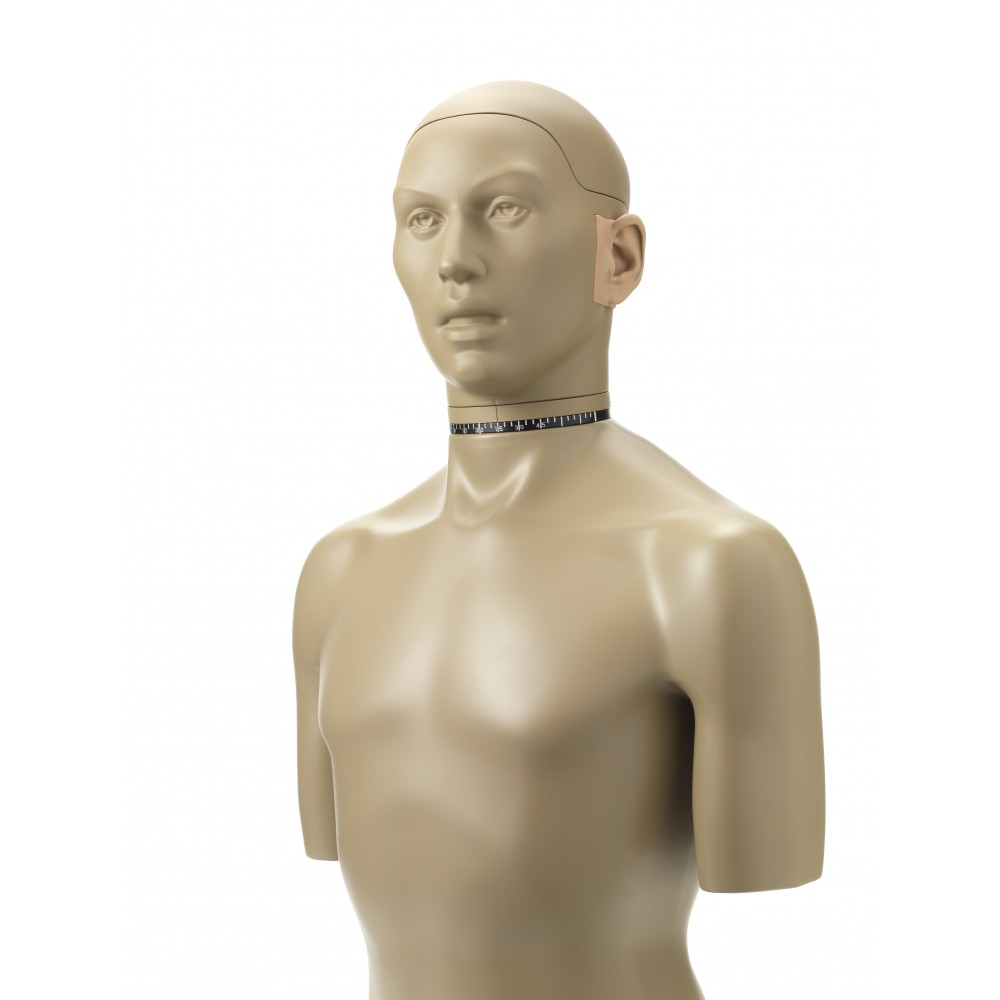
\includegraphics[width=0.22\textwidth]{figure/chapter2/Kemar2.jpg}}
\hfill
\subfigure[]{
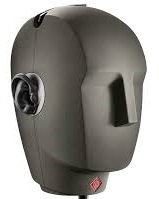
\includegraphics[width=0.17\textwidth]{figure/chapter2/Neumann_KU100.jpg}}
\hfill
\subfigure[]{
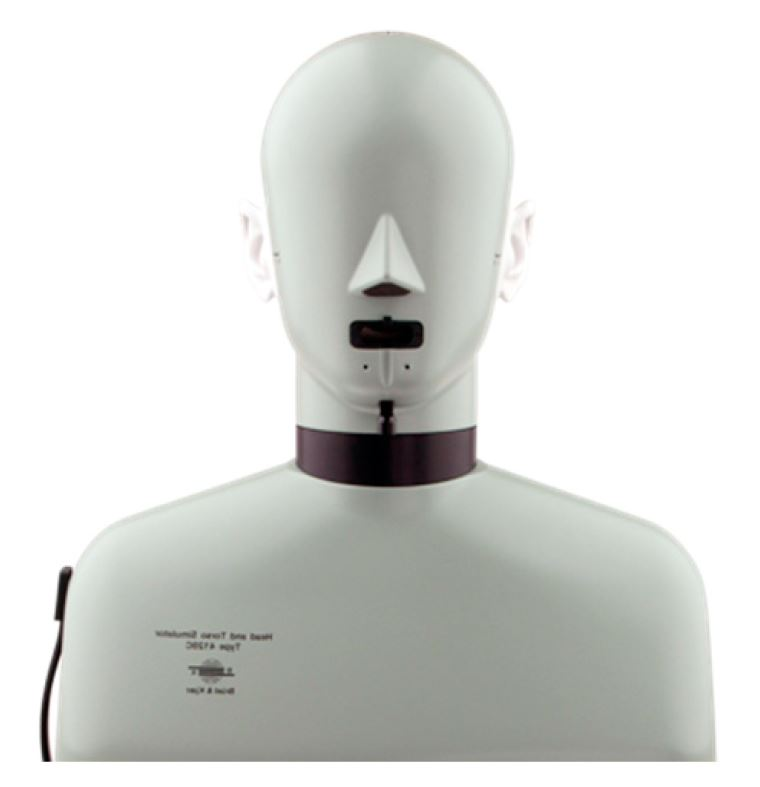
\includegraphics[width=0.21\textwidth]{figure/chapter2/HATS.jpg}}
\hfill
\subfigure[]{
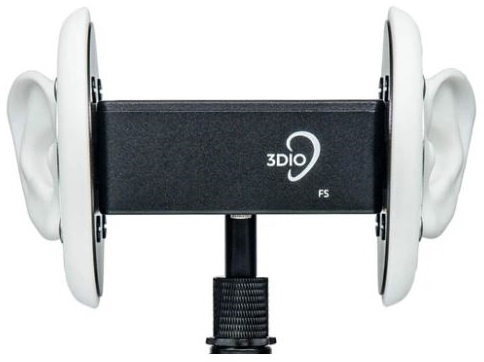
\includegraphics[width=0.21\textwidth]{figure/chapter2/3Diomicrophone.jpg}}
\caption{双耳录音设备,(a)~KEMAR,(b)~Neumann~KU-100,(c)~HATS,(d)~3Dio}
\label{fig:binaural_recording}
\end{figure}


一些广泛使用的双耳录音设备包括仿真人头KEMAR\tcite{KEMAR}、
Neumann~KU-100~\tcite{Neumann_KU100}、头部和躯干模拟器~HATS~\tcite{HATS}~和~3~Dio~自由空间双耳麦克风~\tcite{3Dio}。其中,KEMAR~已被广泛用于头相关传递函数~HRTF~(头相关脉冲响应~HRIR)~和双耳房间脉冲响应~BRIR~的测量,例如麻省理工学院~\tcite{hrtf_MIT}、华南理工大学~\tcite{2013Report}~以及柏林工业大学~\tcite{2011A}。Neumann~KU-100~仅包含了人类头部的结构特征,这种设计便于携带,可以捕获头部和耳廓带来的空间信息,但由于躯干的缺失,肩部所对应的空间线索没有包含在录制的双耳信号中,这一缺陷可能会降低俯仰角线索的强度,从而限制了声音的空间捕捉范围。HATS~的结构与~KEMAR~类似,但其对人体的物理重现精度稍差。 3~Dio自由空间双耳麦克风使用两个仿真人耳进行双耳录音,其间距与人头尺寸相似,但并未考虑头部和躯干对声波的反射和散射。

尽管许多人认为双耳录音是捕捉三维声音和空间线索的最令人信服的方法,但它们的一个限制是,采集的声像代表一个固定的视角。换句话说,一旦声场景被采集,听者就不能转动头部与环境进行互动。相比于静态聆听模式,涉及头部跟踪的交互式系统具有显著的优势,不仅可以创建更加真实和身临其境的聆听环境,还可以提高定位精度,减少前/后和上下混淆~\tcite{2004The}\tcite{2001Direct}。目前已有许多可用的技术来跟踪听众的位置,例如惯性传感器(加速度计、陀螺仪)、声学跟踪、光学跟踪和磁跟踪。


运动跟踪双耳(Motion-tracked~Binaural~,MTB) 是由~Algazi Duda~和~Thompson~于~2004~年提出的一种方法~\tcite{book_immersive}\tcite{review_headphone_spatial},作为一种新的双耳声音捕捉和再现方法,在双耳录音的基础上进行推广,保留了动态头部运动线索,允许听者移动头部,获得以听者为中心的声像。基于使用假人头模型进行声音捕捉的概念,MTB~使用分布在一个接近人头的球体表面上的麦克风获取双耳信号。实际系统中使用一个圆形麦克风阵列,直径设定为人体平均头部直径,如图~\ref{fig:MTB&Omni}~(a)~所示。在回放过程中跟踪听者头部在水平面上的运动,使用头部跟踪器来确定最接近听者耳朵位置的麦克风,并且集成有信号插值模块,可以更有效地获取双耳信号。
如果听者耳朵所在位置碰巧与麦克风位置吻合,来自该麦克风的信号直接发送至耳机;如果耳朵在两个麦克风之间,信号经过插值后发送至耳机。

\begin{figure}[H]
\centering
\subfigure[]{
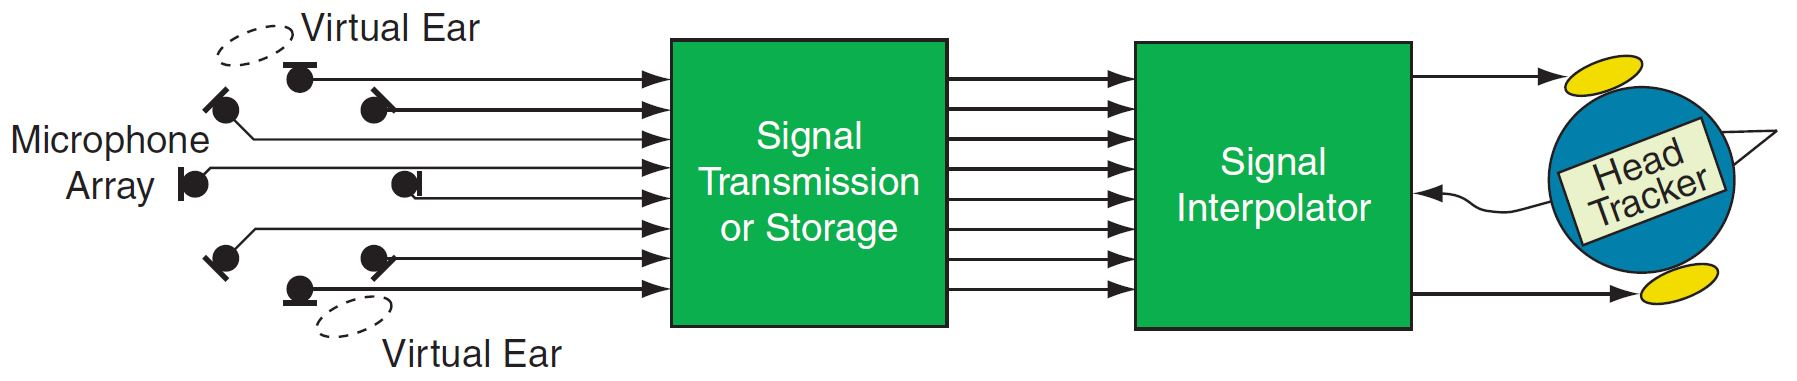
\includegraphics[width=0.74\textwidth]{figure/chapter2/MTB.jpg}}
\hfill
\subfigure[]{

\includegraphics[width=0.22\textwidth]{figure/chapter1/Omni.jpg}}
\caption{多自由度双耳录音设备:(a)~MTB~\tcite{review_headphone_spatial};(b)~Omni }
\label{fig:MTB&Omni}
\end{figure}


但是,MTB~方法并非没有限制。由于麦克风没有配备人造外耳或耳廓,所以信号缺乏与听者仰角定位相关的谱线索。如图~\ref{fig:MTB&Omni}~(b)~所示,Omni~双耳麦克风与~MTB~类似,是由~3Dio~发展而来。其包含沿正方形放置的四对耳廓,每一边均配备了一个左耳耳廓和右耳耳廓,允许从四个不同的角度捕获双耳信号,即可以同时捕获头部朝向四个方向的双耳信号。类似于~MTB,在重放过程中,可以根据听者的方向调整输出双耳信号。


双耳录音的限制包括以下两点:一是其设备尺寸较大,便携性差。二是仿真人头录音要在个体差异和良好的空间感知之间折中。每个人身体都有独特的尺寸和形状特征,因此直接使用仿真人头录音代替人耳可能会造成空间混淆,特别是在仰角定位方面。这个问题也被称为~HRTF~的个性化差异,是~HRTF~的特征之一。


\subsection{双耳合成}
%%%%%%%%  信号处理
%%%%%%% 双耳合成(binaural synthesis)

一般来说,双耳信号可以分为两个主要成分,一是声音从声源传播到听者所在的位置,二是听者头部等生理结构对声波的影响。“双耳”一词专指进入听者耳朵的双声道声音经过了一系列旨在模仿人类定位的线索的综合滤波。这些线索可以被自然地叠加(例如双耳录音),也可以通过信号处理的方式获得(例如双耳合成)。自从~1989~年~Wightman~和~Kistler~采用信号处理的方法在耳机重放中模拟出三维空间虚拟源~\tcite{wightman1989headphone_a}\tcite{wightman1989headphone_b}以来,虚拟听觉重放的研究得到了很大的发展,成为国际上空间声的研究热点,并在许多领域得到了广泛的应用~\tcite{3D_Sound_VR}\tcite{wightman2005measurement}\tcite{book_xiebosun},例如在电脑游戏和军事训练系统中遇到的虚拟声学环境。本节将对现有的双耳合成方法进行介绍。

头相关传递函数~HRTF~在双耳合成中至关重要,是双耳空间研究及虚拟听觉应用的核心问题。其描述了听者的头部、躯干和耳廓等生理结构对入射声波的综合滤波,包含了双耳声压的各种空间线索,尤其是人耳听觉系统对声源进行精确定位的关键线索,例如~Rayleigh~双因素理论中的双耳时间差和双耳声级差,耳廓所带来的单耳因素~——~谱因素。HRTF~的时域表示为头相关脉冲响应~HRIR。
% 1907~年,Rayleigh~提出的双因素理论表明,双耳声音的方位感知主要依赖于双耳时间差~ITD~和双耳声级差 ~IID~这两个线索。

简单的双耳合成是通过对声源的单声道信号卷积左右耳的~HRIR~来实现。如上所述,一对左右耳~HRIR~包含了听者感知声源方位所必要的空间线索。当我们将包含在~HRIR~中的线索叠加在一个声源信号上,可以创建一个位于听者耳道入口处的双耳信号,由此产生了声音似乎来自~HRIR~所对应方位的一种错觉。

用于双耳合成的~HRIR~可以是通用的、单独测量的、从数据库中选择的和/或定制的,其中许多~HRIR~数据库是在无回声环境中测量的。也可以捕捉扬声器、室内声学和听者~HRIR~的组合特性,从而得到双耳房间脉冲响应~BRIR。同样,通过卷积将左右耳的~BRIR~和扬声器播放信号相结合,即可通过耳机重现一个在房间内的虚拟声源,使感知到的虚拟声像等效于房间里的真实扬声器。

% 自然界是一个不断变化的环境,声源与听者的相对位置可以通过以下两种方式来修改:1)声源位置的改变,2)听者位置或方向的改变。因此
在渲染过程中,当声源位置相对于听者发生动态变化时,要想给听者产生连续空间位置变化的主观印象,而不是突然的声像变化,必须经常更新虚拟声源的位置并使用相应的~HRIR~和~BRIR~滤波器。为了在空间上产生均匀的运动状态,HRIR~和~BRIR~必须在两个或多个离散测量的位置之间进行插值,以获取各个位置的~HRTF。目前已经有多种方法和技术应用于时域和频域的插值,例如简单局部线性插值、主成分分析(PCA)、Karhunen Loeve~展开、小波域表示和球谐函数分解。

%%%%%

上述信号处理方法需要已知声源位置和相应的驱动信号,常用于~VR~产生虚拟声学环境。 对于捕捉的自然声场, 经常存在多个声源的叠加,此时需要先对采集信号进行方位估计和声源分离。该方法的运算复杂度较高,且估计误差会降低双耳信号的质量。
有一些先进的方法提出对整个声场进行统一处理,避免了方位估计和对多个声源的单独处理,降低复杂声场景下的运算复杂度,同时提升空间音频的效果。其中,Ambisonics~技术已经在物理声场重建领域占据重要地位,现有的部分双耳渲染技术在其基础上进行~\tcite{davis2005high}\tcite{2012All}\tcite{20033D}\tcite{JieruChen_CSMT}。

%%%% AMBISONICS

1973~年,Michael Gerzon~首次提出~Ambisonics~\tcite{gerzon1973}~技术,使用球谐基函数对来自某采样点周围各个方向的声场进行编码和重建。Ambisonic~技术最大的优点是其编码与播放系统无关,因此在重建过程中非常灵活。最初,Michael~Gerzon~和~Peter~Craven~发明了著名的声场麦克风,使用四个麦克风实现入射声场的一阶近似,包括指向~x、y、z~轴的八字形麦克风和一个全向型麦克风进行空间三维录音,分别采集声场的前后、左右、上下和全向信息,即~$X$、$Y$、$Z$、$W$~分量,这四个正交的分量信号被称为~B~格式音频信号。

由于一阶的~Ambisonics~系统使用低阶截断的球谐分解,所获取的声场空间信息不足,不能达到声场重建中完美的沉浸式体验效果,因此高阶~Ambisonics~引起了广泛关注。更高阶的~Ambisonics~系统(HOA)使用额外的麦克风,在数学上进行更高阶次的球谐波展开来实现声场的更精确逼近,重现效果较为理想,最佳听音区和可实现的音频带宽得以提高。目前在技术上比较成熟的~Ambisonics~话筒有~CoreSound~的~TetraMic、TSL~的声场麦克风~SPS200~,以及可进行高阶~Ambisonics~录制的~Eigenmike~球形话筒~\tcite{microphone},如图~\ref{fig:Ambisonics_microphone} 所示。

\begin{figure}[H]
\centering
\includegraphics[width=0.75\textwidth]{figure/chapter2/Ambisonics_microphone_new.eps}
\caption{Ambisonics~麦克风}
\label{fig:Ambisonics_microphone}
\end{figure}


双耳渲染技术对~Ambisonics~方法进行移植,和虚拟扬声器方法相结合,获取双耳信号。基于耳机的虚拟扬声器方法的目的是仿真听者在含有一个或多个扬声器的场景中的听感。对所有虚拟扬声器的声源信号卷积相对应方位的左右耳~HRIRs,并进行叠加,以获取综合的双耳信号。虚拟扬声器方法不仅可以和~Ambisonics~技术进行结合,还可以与~5.1、 7.1、10.2、22.2~等多通道环绕声相结合,创建虚拟听觉 。

但是基于~Ambisonics~的虚拟扬声器方法会带来一些问题:一是不同的虚拟扬声器数目和位置会对所获取的双耳信号带来影响,二是扬声器所在位置的声像会不可避免地被加重。

近年来,球形麦克风阵列在声场录制及重放领域中日益普及。球面阵列的使用自然导致在球面谐波(Spherical Harmonics,SH)域中进行 三维声场的处理和分析。
1998~年,Evans~等人~\tcite{1998Analyzing}~首次提出了用球谐函数来表示~HRTF~的方法,接着一些新的双耳渲染工作在球谐域进行~\tcite{Bernsch2014Binaural}\tcite{sheaffer2014rendering}\tcite{2018Binaural}\tcite{2019Perceptual}。
其核心思想是不仅将声场在球谐域进行表示,同时将~HRTF~在球谐域展开,并直接在球谐域中进行渲染。

在球谐域渲染双耳信号的优点在于能够直接使用现有的球谐域算法来处理声场或相应的~HRTFs,例如波束形成、定位等。在球谐域实现听者追踪时,只需要对原始声场乘以一个旋转因子即可实现对声场的转向~\tcite{2008Spherical},无需传统算法中的~HRTF~匹配和插值。
相比于基于~Ambisonics~的虚拟扬声器方法来说,该方法无需解码到虚拟扬声器这一步骤,避免了虚拟扬声器数目和位置对听感的影响。

为了精确地使用球谐函数表示声场和~HRTF,通常需要使用高阶展开。然而实际系统中由于麦克风数量有限,导致声场的阶次较低,一般实际系统中小于~5~阶~\tcite{2018Binaural}。而对于现有的~HRTF~数据库来说,其球面采样点较多,可以实现较高的分解阶次。Zhang~等人~\tcite{2016Insights}~对~HRTF~的空间维度进行了研究,得出的结论是,要想对高达~15~kHz~的~HRTF~进行精确的物理表征,大约需要~34~阶。

声场和头相关传递函数~HRTF~之间存在不匹配性,最简单直接的方法是对~HRTF~进行低阶截断,与声场阶次保持一致。但是现有的低阶双耳渲染算法在提供高保真空间声方面仍受到很多限制。HRTF~的直接低阶截断会导致高频能量损失,带来一定的误差,导致空间分辨率受限,直接影响对声源方位的感知、外化~(externalization)、感知声源宽度和音色等~\tcite{sheaffer2014rendering}\tcite{2013Spatial}\tcite{2015Efficient}\tcite{2017equalization}。

现有的一些改进方法主要集中在~HRTF~的预处理方面,例如,通过使用时间对准或相位对准~\tcite{1998Analyzing},最小相位表示~\tcite{2015Efficient},或方向均衡~\tcite{2019Directional}~等。文献~\cite{2018comparison}~对现有的方法归纳总结,主要分为单纯基于复谱的方法和复合方法,其中复合方法分别处理~HRTF~的绝对值和相位。包括相位上的频域解卷积、空域解卷积、时间对准,幅度上的取对数谱,以及对复频谱进行平滑,并且可以相互结合,如表~\ref{tab.pre_processing}~所示。


\begin{table}[H]
\caption{HRTF 预处理方法}
\centering
\begin{tabular}{|c|c|c|}
\hline
方法 & 预处理对象 & 预处理方法 \\
\hline
$H_{a}$ & 复频谱 & 时间对准 \\
$H_{s m}$ & 复频谱 & 平滑 \\
$|H|$ & 幅度谱 & 无 \\
$|H|_{\mathrm{dB}}$ & 幅度谱 & 取对数 \\
$\left|H_{s m}\right|$ & 幅度谱 & 平滑 \\
$\left|H_{s m}\right| \mathrm{d} \mathrm{B}$ & 幅度谱 & 平滑,取对数\\
$\angle_{f} H$ & 相位 & 频域解卷绕 \\
$\angle_{s} H$ & 相位 & 空域解卷绕 \\
$\angle_{f} H_{s m}$ & 相位 & 平滑,频域解卷绕\\
\hline
\end{tabular}
\label{tab.pre_processing}
\end{table}


基于双耳对准的~HRTF~预处理方法(时间对准、相位对准)已被证明是一种有效降低~HRTF~球谐分解阶次的稳健方法,有很多工作基于此进行。

2018年,Zaunschirm~等人的另一项研究~\tcite{2018Binaural}~也提出了改善球谐域双耳渲染算法中的~HRTF~阶次问题。通过去除高频~HRTF~的线性相位成分,实现了频率相关的时间对准的~HRTF~预处理方法,并在再现信号上添加扩散场约束。2019~年,Zamir Ben-Hur~等人~\tcite{2019Efficient}~将相位对准预处理和新的稀疏采样方式相结合,提出了一种有效的~HRTF~表示方法。该方法能够在相对较少的方向上测量~HRTF,并通过精确的插值重建高空间分辨率的~HRTF。结果表明,该方法仅需要~100~个测量方向的稀疏~HRTF~采样,不到全采样所需测量次数的~10$\%$。

2020~年,Zamir Ben-Hur~将对~HRTF~引入相位对准这种有效的表示融入到整个双耳渲染过程中~\tcite{ben2020binaural},提出了一个新的概念——双耳~Ambisonics~信号。该信号表示左右耳所在位置的声场~Ambisonics~表示,可以直接录制某场景下两个耳朵处的声场,例如使用两个分别位于左右耳处的~Eigenmike~或声场麦克风,也可以由录制声场计算得到左右耳位置出的声场分量,计算原理与~HRTF~进行双耳对准的逆过程相似。

除此之外,还有一些~HRTF~预处理方法通过对~HRTF~的稀疏采样降低球谐分解的阶次,也有部分方法主要集中在对双耳信号的频谱补偿方面。


2014年,Bernschütz~等人对~HRTF~数据库进行空间重采样~\tcite{Bernsch2014Binaural},根据所需的阶次设定相对应的低阶复合网格,有效的采样网格可以减少音色失真。采样方式包括等角高斯采样和列别捷夫采样,若~HRTF~数据库不包含所选取的采样点,则需要引入插值的方法获取。


2017~年,Zamir Ben-Hur~等人提出了一种将低~SH~阶双耳信号的频谱校正为高~SH~阶频谱的均衡滤波器~\tcite{2017equalization},使原始双耳信号的频谱分布更为均匀。该方法以刚性球为模型,通过计算高阶扩散场与低阶截断扩散场的比值获取均衡滤波器,从而减小阶次降低对~HRTF~所带来的影响。所提出的滤波方法能够有效地恢复截断后的双耳信号的音色成分,同时保留甚至改善了信号的一些空间特性。结果显示,当使用均衡滤波器时,再现信号的空间感知能力显著改善,双耳声音的音色得以校正。另外,虚拟源被认为完全外化。


2019~年~Christoph Hold~等人提议通过补偿滤波器和球谐域渐变来校正音色~\tcite{2019Improving}~。之前的研究直接对~HRTF~进行低阶截断,这相当于一个矩形窗。该方法在~HRTF~在截断过程中进行加窗,降低直接使用矩形窗进行阶次截断所引入的旁瓣,并且和均衡滤波器相结合。结果表明,所提出的方法可以减少音色损失,从而改善音频的感知质量。

还有一部分工作对现有的~HRTF~预处理方法进行比较和进一步验证,例如~Brinkmann~等人在~2018~年和~Lubeck~等人在~2019、2020~年的几项研究~\tcite{2018comparison}\tcite{lubeck2019perceptual}\tcite{Tim2020Perceptual}~验证了各种~HRTF~预处理方法对双耳信号在感知方面的改善。





\section{研究内容与论文结构}

\subsection{研究内容及创新点}

本论文聚焦于球谐域的双耳渲染技术。尽管这一领域已经取得了重大进展,但基于低阶球谐的高质量双耳渲染算法仍然是一个值得探索的问题。

对于球谐域双耳渲染算法来说,其包含两个同等重要的部分,声场和~HRTF。二者之间存在阶次和尺寸等不匹配问题,直接基于低阶~HRTF~球谐分解的双耳渲染算法会对双耳信号带来众多感知方面的损失。实验研究表明,当双耳信号以更高的球谐波阶次进行重构时,对声源的感知会更清晰和更外化,使用更高的球谐波阶构建双耳表征将导致外部的、更窄的、更远的声像,以及更平衡的音色。
%文献~\cite{2013Spatial}~在球型麦克风阵列录制声场和双耳合成感知之间建立了一个更加清晰的关系。

近年来许多学者对低阶球谐分解的双耳渲染算法加以改进,但这些方法都是从~HRTF~角度出发。本文不仅从~HRTF~预处理的角度出发,并且在声场层面对现有的双耳渲染算法加以改进,创新性提出了一种新的声场扩阶理论,并且将声场扩阶理论、头相关传递函数预处理和基于球谐分解的双耳渲染算法相结合,实现了基于声场扩阶的双耳渲染算法。 该声场扩阶理论对麦克风阵列的采集声场进行分析,将入射声场分解为直达波和混响场的叠加。根据直达波入射方向进行空间加窗处理,可以实现声场分量的阶次提升,同时扩大控制区域的半径。


\subsection{论文结构安排}

论文共分为六个章节,各章节的主要内容如下:
\newpage

\par
本章(第一章)为绪论。首先对增强现实下双耳渲染技术的研究背景及可预见的应用进行了简单的介绍,接下来对现有的双耳渲染实现方法加以详细阐述,最后说明了本文的研究内容、创新点与论文结构安排。
\par
第二章为双耳渲染算法。本章对三种典型的双耳渲染算法的原理进行详细介绍,其中包含本文所关注的基于球谐分解的双耳渲染算法,并给出了双耳渲染中至关重要的头相关传递函数和声场的球谐分解等基础知识,为后续工作奠定理论基础。
\par
第三章为基于~HRTF~球谐分解的双耳渲染算法。本章首先详细介绍了声场和头相关传递函数~HRTF~的球谐分量求解方法,并对本文所采用的~HRTF~预处理方法进行介绍,最后通过实验验证了预处理算法的有效性。
\par
第四章为基于声场扩阶的双耳渲染算法。本章首先对信号模型和球谐域~MUSIC~定位算法进行介绍,其次从有界线性算子出发,对通过空域加窗实现声场阶次提升的方法进行详细推导,最后将声场扩阶和~HRTF~预处理方法相结合,给出总体算法框架。
\par
第五章为实验结果及分析 。本章首先对评价指标及其计算方法加以介绍,其次在消声室和混响环境下,将对标算法和本文所提出的算法进行对比和分析,验证本算法的优越性。
\par
第六章为全文总结。对论文的研究内容进行归纳和总结。

